\documentclass{article}
\usepackage[utf8]{inputenc}
\usepackage{blindtext}
\usepackage{enumitem}
\usepackage{graphicx}
\graphicspath{ {images/} }

\title{\textbf{Werewolves of Miller's Hollow}}
\author{João Silva\\
		Marcelo Ferreira\\
		Miriam Gonçalves}
\date{31 October, 2017}
\begin{document}

\maketitle
\section{Examination Paper}
\subsection{Scenario Description}
\textit{Werewolves of Miller’s Hollow} game is based on the russian game called “Mafia” and can be played by groups between eight and eighteen people. 
Game Components (24 roles):
\begin{itemize}
	\item 4 Werewolves; 	
	\item 13 Ordinary Townsfolk and there are 8 different kinds of Townsperson: 
	\begin{itemize}
		\item 1 Fortune Teller - can see the true personality of one player each night, with its capacities it will help the townsfolk to find  correctly the identity of the werewolves;
		\item 1 Thief - if this role is used, two additional ordinary Townsfolk are added at the beginning of the game. Afterwards two cards are placed face down in the center of the table, during the preliminary turn of the first night, this player looks at these two cards and may trade his/her cards with one of them. However if both of the cards are werewolves, the Thief must trade his card with one of them. If this player takes on of the extra cards, he/she assumes the role of this player for the rest of this character for the rest of the game;
		\item 1 Hunter - if the hunter is killed during the game he can retaliate by eliminating another player;
		\item 1 Cupido - got the ability to make any two people fall instantly in love for the rest of the game, these two people are designated during the first night of the game. If one of the lovers die, the other must kills him/herself immediatly. In case of one of the lovers being a townsperson and the other a werewolf, they must eliminate all the other players from the game to live in love and peace;
		\item 1 Witch - make two kind of powerful potions: one is the \textit{healing} potion that can resurrect a player killed by a werewolf, the other is a \textit{poison} that kill a player during the night. Each potion can be used only once per game and use them on him/herself;
		\item 1 Little Girl -this character can open her eyes during the night to spy on the werewolves, but if she gets caught by them she immediatly dies instead of the designated victim;
		\item 1 Sheriff - this role is entrusted to one of the players, this person is elected by the townsfolk and once elected this player cannot refuse the honor. Afterwards this player's votes count as two votes. If this player dies during the game he/she must name his/her successor.
	\end{itemize}
\end{itemize}

For each number of players there are different combinations of roles:
\begin{center}
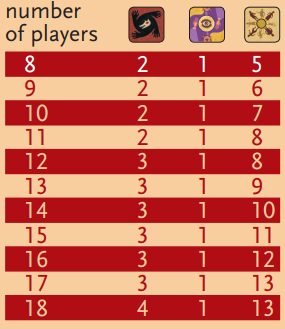
\includegraphics[scale=0.6]{playermix}
\end{center}

\setlength{\parindent}{0cm}There are two phases in the game: 
\begin{itemize}
	\item the night - when werewolves devour and kill one Townsperson (that person is eliminated from the game);
	\item the day - the townsfolk try to conceal their identity and discover who the werewolves are by voting on a suspect who is eliminated from the game.	
\end{itemize}

The game ends when:
\begin{itemize}
	\item the townsfolk manage to eliminate all the werewolves;
	\item the werewolves kill the last townsperson;
	\item the lovers are the surviving townsperson/werewolf pair, and the all other players are dead; 
\end{itemize}
\subsection{Objectives}
This work has the goal to create the game \textit{Werewolves of Miller’s Hollow} following all the rules of the game, creating the different roles through different types of agents and evaluating their performance to see what agents are the most adequates for each role. 
\subsection{Expected results and evaluation form}

\section{Platform/Tool}
\subsection{What it is used for}
\subsection{Description of the main characteristics}
\subsection{Highlight of the main features for the work}
\section{Specification}

\subsection{Agents}
In order for the game to take place, agents need to assume all the necessary parts. For our purposes we consider each role to be a different type of agent. As such, at the highest level of abstraction, there are two main roles: The players and the game coordinator.

Players are responsible to play the actual game. They must negotiate with other players, collaborate with their team and compete with the opposing team with the ultimate purpose of winning the game. How they go about achieving this is dependant on which role they play. In practice, character agents will be a subclass of the abstract player agent that implement their specific behaviors:

The game coordinator is responsible for controlling the flow of the game and relaying information about the environment to the players. It's the only purpose is to take the game all the way to completion.

\begin{center}
	\begin{tabular}{ p{3cm} l p{5cm} }
	Agent & Inherits & Description \\
	\hline
	Game Coordinator & N/A & Responsible for controlling the game flow\\
	Player & N/A \\
	Werewolf & Player & Plays the role of the werewolf \\
	Ordinary Townsperson & Player & Plays the role of the townsperson \\
	Fortune Teller & Player & Plays the role of the fortune teller \\
	Thief & Player & Plays the role of the thief \\
	Hunter & Player & Plays the role of the hunter \\
	Cupido & Player & Plays the role of the cupido \\
	Witch & Player & Plays the role of the witch \\
	Little Girl & Player & Plays the role of the little girl \\
	Sheriff & Player & Plays the role of the sheriff \\
	\end{tabular}
\end{center}

\subsection{Environment}
In order to formalize the agent's architecture let us first consider the environment in which the agents will live in. The game's environment is the game state in each round; the number of agents still in play and their roles. According to Russell and Norvig (Russell and Norvig, 2010, p.42), an environment can be either: Single-Agent or Multi-Agent; Fully Observable or Partially Observable; Deterministic or Non-deterministic; Episodic or Sequential; Static or Dynamic; Discrete or Continuous; and Known or Unknown. We'll address each of these in order.

The environment in which our agents interact is obviously multiagent, considering that the smallest number of agents required to play the game is eight. Not only that, it is a partially cooperative multiagent system given that agents on the same team (the townsfolk for example) must cooperate in order to win the game. But it is also a partially competitive multiagent system because, in the end, only one team is victorious; either the townsfolk kill all the werewolves, or the werewolves kill all the townsfolk.

Russell and Norvig describe a fully observable environment as an environment in which "the sensors detect all aspects that are relevant to the choice of action". That is decidedly not true in the environment of our game since agents purposely withhold information from each other. For example, a werewolf would not (except for strategic reasons) let others know that he is a werewolf, as that would get him lynched. As such the environment is partially observable; the agents cannot get reliable and up-to-date information regarding the environment from their sensors alone.

In a deterministic environment, the next state of the environment can be fully determined given only the current state and the action executed by the agent. Because of that, it is not obvious whether the environment of our game is deterministic or non-deterministic. In one hand there is uncertainty in the outcome of the actions of any agent; Say agent A decided that agent B is definitely a werewolf and votes to lynch them, but because the other agents do not agree with A, agent C is lynched instead. In this case, the agent action (vote to lynch B) resulted in B being lynched but had the other agents agreed with A then agent B would be lynched instead. It's then clear that the same action from an agent could result in more than one outcome, suggesting a non-deterministic environment. However, because the uncertainty arises purely from the actions of other agents a case can be made that the environment is actually deterministic in that the same actions from all the agents in the system will always result in the same outcome.

Deciding whether the environment is episodic or sequential is also not quite a trivial affair. At a glance we can say that each round is an episode, meaning that actions taken in each round are independent and do not depend on actions taken in previous rounds. But once we look closer it appears that that hypothesis does not hold; that some actions can have long-lasting consequences. For example, if the agents decide to kill the Fortune Teller early in the game, then from then on they have one less source of information from which to base their decisions on, affecting the way those decisions are made. The environment can then be considered sequential.

A somewhat easier property of the environment to identify is whether it is static or dynamic. In our game, the state of the environment does not change while an agent is deliberating. The game is played in turns, and every environment altering decision is made once at the end of each turn by all agents, making the environment static.

Discrete environments have a finite number of percepts and actions. This seems to be in line with the environment our game takes place in: The game is turn-based (or, in other words, is not a continuous-time problem) and there is only a finite number of states the environment can be in. 

The last property of the environment is related to the state of knowledge of an agent about the laws or rules of the environment. In the case of our game every agent is aware of the game's rules (otherwise they would have to learn as they played, which is very hard if not impossible given no base knowledge about the game) which means that the environment is known.

This makes our environment multiagent, partially observable, deterministic, sequential, static, discrete and known.

\section{Resources}
\subsection{Bibliography}
\subsection{Software}
\end{document}